\section{问题一：近地层结构、天气过程与统一关联排序}
\subsection{问题口径与分析范围}
题面要求依据MET、RADM、SOIL与FLUX四类逐时观测，分析高寒山区近地层结构、天气过程和极端事件，并给出与本次泥石流关联最高的五个特征。本文将诊断与排序分开：前者描述边界层和能量过程的结构，后者在固定候选池和同季匹配背景下判断本次冲击前哪个环境量最异常。目前只有一次确证事件，且没有完整非灾目录，因此结果限于环境关联排序，不涉及灾害发生概率、总体因果效应或分类AUC。正式前五指：在统一候选池中，按事件前环境窗相对同季历史窗的稳健异常、经相关簇去冗余后的五个代表量。

\subsection{五层静力订正与稳定度诊断}
梯度观测高度为1、2、4、10、20米。MET表头只给一个Pressure字段，未给气压传感器参考高度；FLUX的PA又缺少安装与校准信息。若把整层气压视为常数，层间压降会进入位温、虚位温和整体理查森数，使稳定度混入压力假设。本文以2米为参考高度的显式工作假设，保持五层温湿与MET气压共同有效，按
\begin{equation}
\frac{\mathrm d\log p}{\mathrm dz}=-\frac{g}{R_dT_v},\qquad
T_v=(T_C+273.15)(1+0.61q)
\end{equation}
作逆虚温分段梯形积分，更新层压三次。每次用当前层压重算比湿、位温和虚位温，再以第三次层压统一重算全部诊断量；第二、三次更新差的中位约$9.1\times10^{-12}$ hPa，最大约$6.5\times10^{-11}$ hPa，说明迭代已收敛，但不构成传感器误差界。

五层共同有效45577小时，占全部49545小时的91.99\%；仅3个可用小时因五层要求被新增剔除。可计算整体$Ri_b$的共同样本为44018小时。位温、虚位温与整体理查森数取
\begin{equation}
\theta_z=T_{K,z}\left(\frac{1000}{p_z}\right)^{0.2857},\quad
\theta_{v,z}=\theta_z(1+0.61q_z),\quad
Ri_b=\frac{g}{\bar\theta_v}
\frac{(\theta_{v,20}-\theta_{v,2})(20-2)}
{(u_{20}-u_2)^2+(v_{20}-v_2)^2},
\end{equation}
其中饱和水汽压采用Bolton式，温度入口为摄氏、位温入口为开尔文，两个入口不混换。切变平方小于$10^{-6}\ \mathrm{m^2/s^2}$时屏蔽并报告比例，不强行赋有限值。

静力订正会实质改变稳定度分类。与“全层同一气压”的对照相比，44018个共同小时中有9016个分类改变，占20.48\%；同压对照的$Ri_b$中位为$-0.0636$，订正后为$-0.0294$，$p05$--$p95$为$-4.343$--$19.647$。订正后的五级频率依次为强不稳定0.2441、不稳定0.3856、中性0.0531、稳定0.0852、强稳定0.2320。两组使用同一批小时，只改变层压处理，故差异不是由样本变化制造的。

逆温按实际温度梯度而非位温梯度定义，操作阈值为0.05 K/(100 m)。总逆温频率为0.4111，夜间0.6007、白天0.2079，呈现夜间辐射降温、白天地表受热增强混合的相对日变化。有效厚度以2米为底层，依次检查2--4、2--10、2--20米的首个$Ri_b=0.25$交点；已出现交点的中位为4米，交点层顶以4米最多（7698小时），10米2392小时、20米1437小时；31116小时在20米内仍未达到0.25，按右删失记录；20米是观测上限，不是真实边界层高度。

\begin{figure}[htbp]\centering
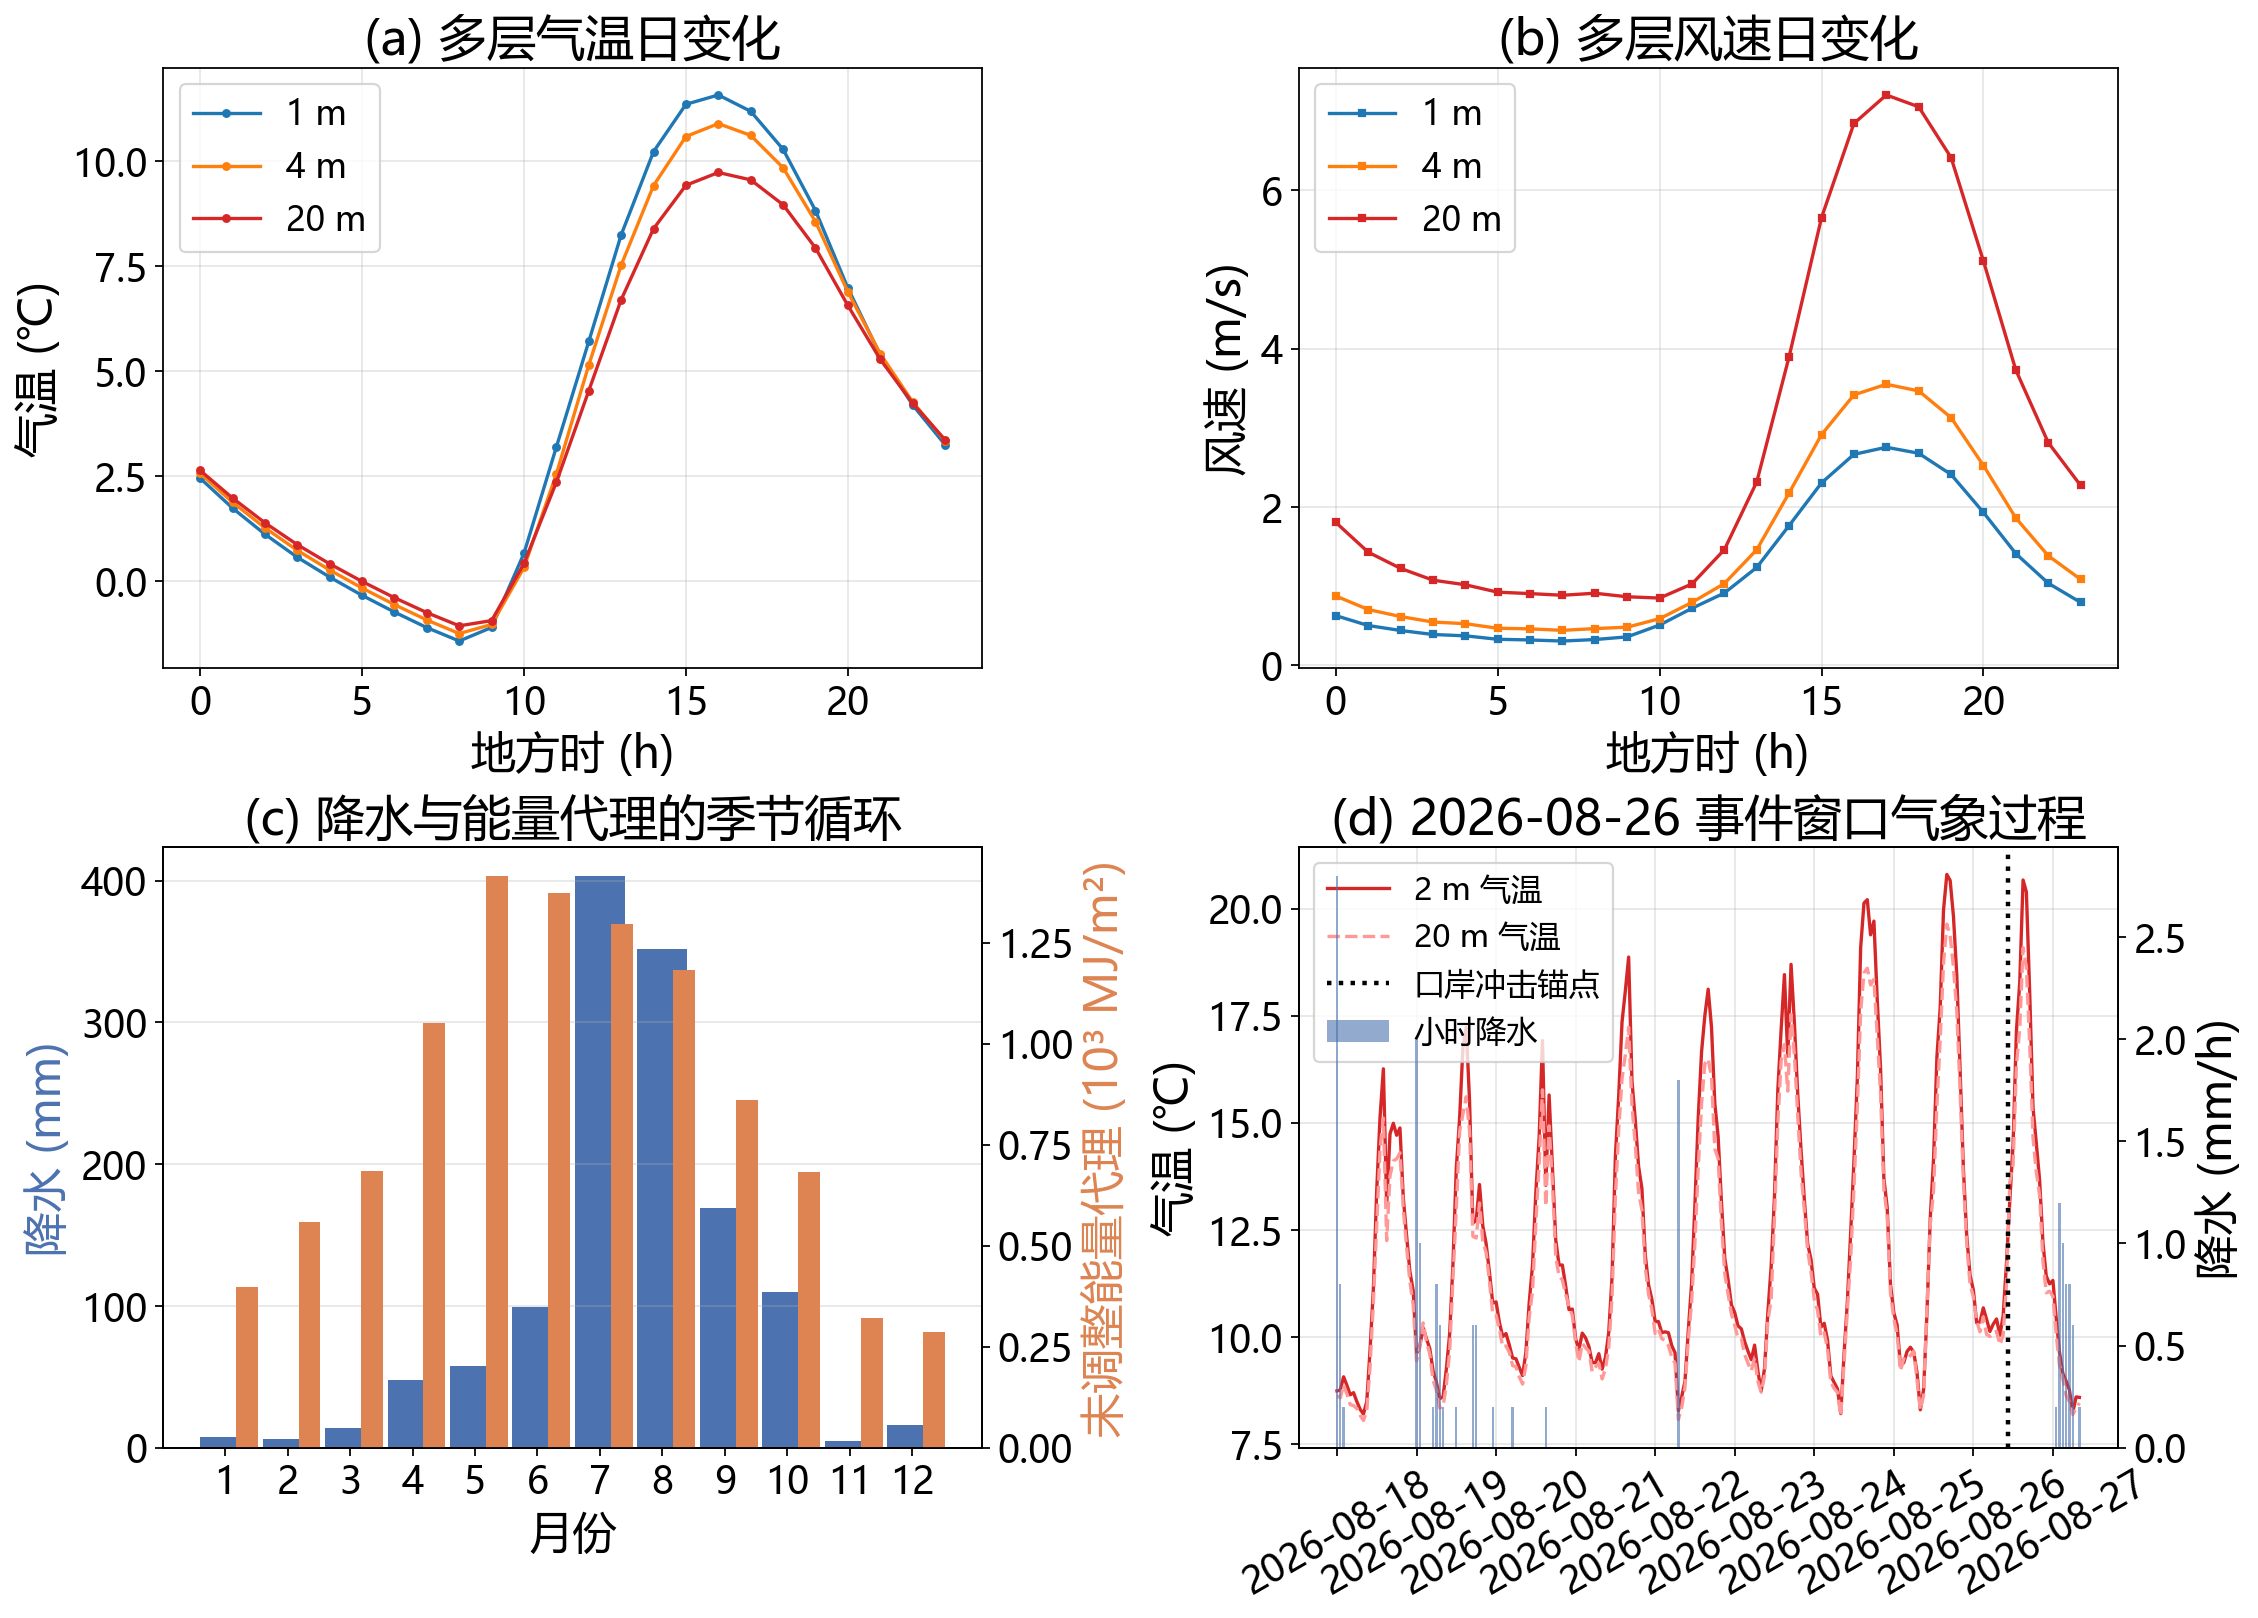
\includegraphics[width=0.78\textwidth]{figures/01_边界层结构.png}
\caption{近地层日变化与事件窗口}
\label{fig:boundary}
\end{figure}

图中季节能量为代理量，事件全日曲线仅用于描述。这些频率受质量码、夜间弱湍流缺测和20米观测上限限制。图\ref{fig:boundary}的日变化是多年统计，不是单个事件的独立控制实验；夜间逆温常见，也不等于每次泥石流都由逆温触发。图\ref{fig:hydrostatic}比较同一批小时上“整层同一气压”与1、2、10、20米参考高度订正的结果，分类改变集中在中性与稳定边界附近。参考高度是工作假设，差异不反映真实传感器高度。

\paperfig{figures/01_静力订正敏感性.png}{0.78}{静力订正敏感性}{fig:hydrostatic}

\subsection{辐射收支、天气过程与极端事件}
用四分量辐射构造$R_n=R_{sd}-R_{su}+R_{ld}-R_{lu}$，反照率只在短波足够大时使用。未调整的小时潜在融化能量为
\begin{equation}
e_m=0.0036[R_n-G-(H+LE)]^+\quad[\mathrm{MJ/m^2\,h^{-1}}],
\qquad [x]^+=\max(x,0).
\label{eq:energy}
\end{equation}
正部约定排除夜间净冷却被误当作负融水。取2021--2025年、$R_n-G>20\ \mathrm{W/m^2}$且四项共同有效的12125小时，回归斜率$\beta_{EC}=0.3343$，而闭合比
\begin{equation}
C=\frac{\sum(H+LE)}{\sum(R_n-G)}=0.4515
\end{equation}
该比值描述能量账本比例，其不确定度由块重采样估计，回归斜率标准误不适用于此。以完整训练年为块重采样500次，$C$的95\%区间为$[0.4441,0.4619]$，无效重采样比例为0。事件相关三日未调整能量合计32.19 MJ/m$^2$；点闭合比调整后为9.35 MJ/m$^2$，两端比值情景约8.85--10.06 MJ/m$^2$。变化远大于数值舍入误差，故基准保留未调整值，调整值只作结构敏感性，不把两者平均为“更真实的消融量”。

将五层气温、湿度、风速和气压组成16维向量，在2021--2025年标准化后作SVD。前三主成分解释方差为53.997\%、30.716\%、11.173\%，达到85\%需要3个模态。第一主成分与融化能量相关0.4304，与24小时降水相关$-0.0964$，故不宜简单命名为降雨模态。另以训练期90\%分位划分强降水、强消融、二者同超和平缓四类；34782个有效小时的比例依次为9.16\%、8.82\%、1.43\%、80.58\%，缺测小时保持未知，不归入平缓型。

极端量采用12小时游程去丛集后的广义帕累托分布。令$Y=X-u>0$，则
\begin{equation}
F_Y(y)=1-\left(1+\xi y/\sigma\right)^{-1/\xi},\qquad
x_T=u+\frac{\sigma}{\xi}\left[(T\lambda_y)^{\xi}-1\right],
\end{equation}
其中$\lambda_y$为独立过程的年次数，暴露年数按有效小时折算；$\xi=0$取连续极限，$\xi<0$时返回水平还须低于有限上界$u-\sigma/\xi$。小时降水97\%分位落在0，正雨小时全部进入尾部；短记录下2年、5年水平只是拟合描述。复合极端主要集中在6--9月，但因缺少多事件起动目录，本文不估计因果风险倍数。

\subsection{31项统一候选关联模型}
正式候选池在求值前固定为31个唯一变量键，家族构成为MET 19项、RADM 5项、SOIL 3项、FLUX 4项。候选覆盖原始气象、温湿与风廓线派生量、辐射能量、土壤状态和湍流通量。小时降水$P$与3小时、24小时累积量是不同时间尺度，不按别名删除；$P_{\max,1h}$与$P$的数值及缺测掩膜逐行相同，只保留$P$。晴空指数和反照率仅白昼有效，固定后分别只有84与82个目标小时，低于135小时门槛；冻融量则因参照窗不足或稳健尺度为零，三项均保留在候选字典中并标为不可排名，其余28项进入正式评分。

题一关联截止为2026-08-26 00:00（非题三08:00业务发布），最后可用标签为前一日22:00。主窗为
\begin{equation}
\mathcal W_{168}=[2026\text{-}08\text{-}18\,23{:}00,
2026\text{-}08\text{-}25\,22{:}00],
\end{equation}
按小时标签$[t,t+1)$计共168小时；72小时敏感性窗取最后72个标签。目标窗和每个候选的参照窗均要求至少达到80\%有效，即主窗不少于135小时，缺测保持为空，不插值或补零。主参照为2021、2023、2024年同积日前后15日内的93个发布窗；2022年因FLUX摩擦速度和观测湍流动能缺测，没有窗口通过共同覆盖门槛，故该年进入逐时相关计算但不进入窗口参照。2025年同历日窗作为无灾害真值的同类日期对照。

对候选$j$和窗长$L$，令目标窗均值为$m_{j,L}$，参照窗均值的中位数和稳健尺度分别为
\begin{equation}
b_{j,L}=\operatorname{median}_r m^{(r)}_{j,L},\qquad
s_{j,L}=1.4826\operatorname{median}_r
\left|m^{(r)}_{j,L}-b_{j,L}\right|,
\end{equation}
并定义$\Delta_{j,L}=m_{j,L}-b_{j,L}$、$Z_{j,L}=\Delta_{j,L}/s_{j,L}$、$A_{j,L}=|Z_{j,L}|$。MAD为零时采用预先规定的$IQR/1.349$回退；回退值仍为零则不排名。同时报告原始单位差、有符号方向和经验尾秩
\begin{equation}
p^{\mathrm{tail}}_{j,L}=
\frac{1+\sum_r\mathbf 1[A^{(r)}_{j,L}\ge A_{j,L}]}{N_{ref}+1},
\end{equation}
该尾秩只是已选参照中的描述量，不是独立检验$p$值；主排序只按$A$降序。

去冗余在2021--2024年6--9月逐对计算Spearman相关。一对候选至少共享200个有效小时才可判定边，$|\rho_s|>0.8$时连边，再取完整连通簇；全部465对均达到共同有效门槛，共同有效小时数的中位为11208小时。31项候选合并为16个连通簇，其中13个含可排名代表。每簇在168小时主评分中只保留$A$最大的可排名候选进入展示，其他成员和完整统计量继续保存。相关簇只解决展示重复，强相关只表示统计关联，不表示机制相同。

\subsection{正式前五与解释}
去冗余后的正式前五见表\ref{tab:q1-top5}，所有方向均为事件窗偏高。前五直接构成题面所问的统一关联排序；代理标签榜和CRITIC榜不再占用“本题答案”。

\begin{table}[htbp]\centering\small
\caption{事件前168小时统一关联榜前五}\label{tab:q1-top5}
\begin{tabular}{@{}c l l c c c@{}}\toprule
次序&变量&家族&$\Delta$（原单位）&$A$&经验尾秩\\\midrule
1&API（前期降水指数）&MET&14.484464&3.829043&0.0106\\
2&$R_n$（净辐射）&RADM&19.928307&2.343641&0.0745\\
3&24小时升温&MET&0.312310&2.234448&0.0957\\
4&VWC（0.1米土壤含水率）&SOIL&0.035295&1.487331&0.1809\\
5&LE（潜热通量）&FLUX&12.883223&1.133226&0.1724\\\bottomrule
\end{tabular}
\end{table}

表中$A$的前三项未舍入值为3.8290425800714973、2.3436406435384014和2.2344476050143953；后两项为1.4873309113872661和1.1332257049823602。

\begin{figure}[htbp]\centering
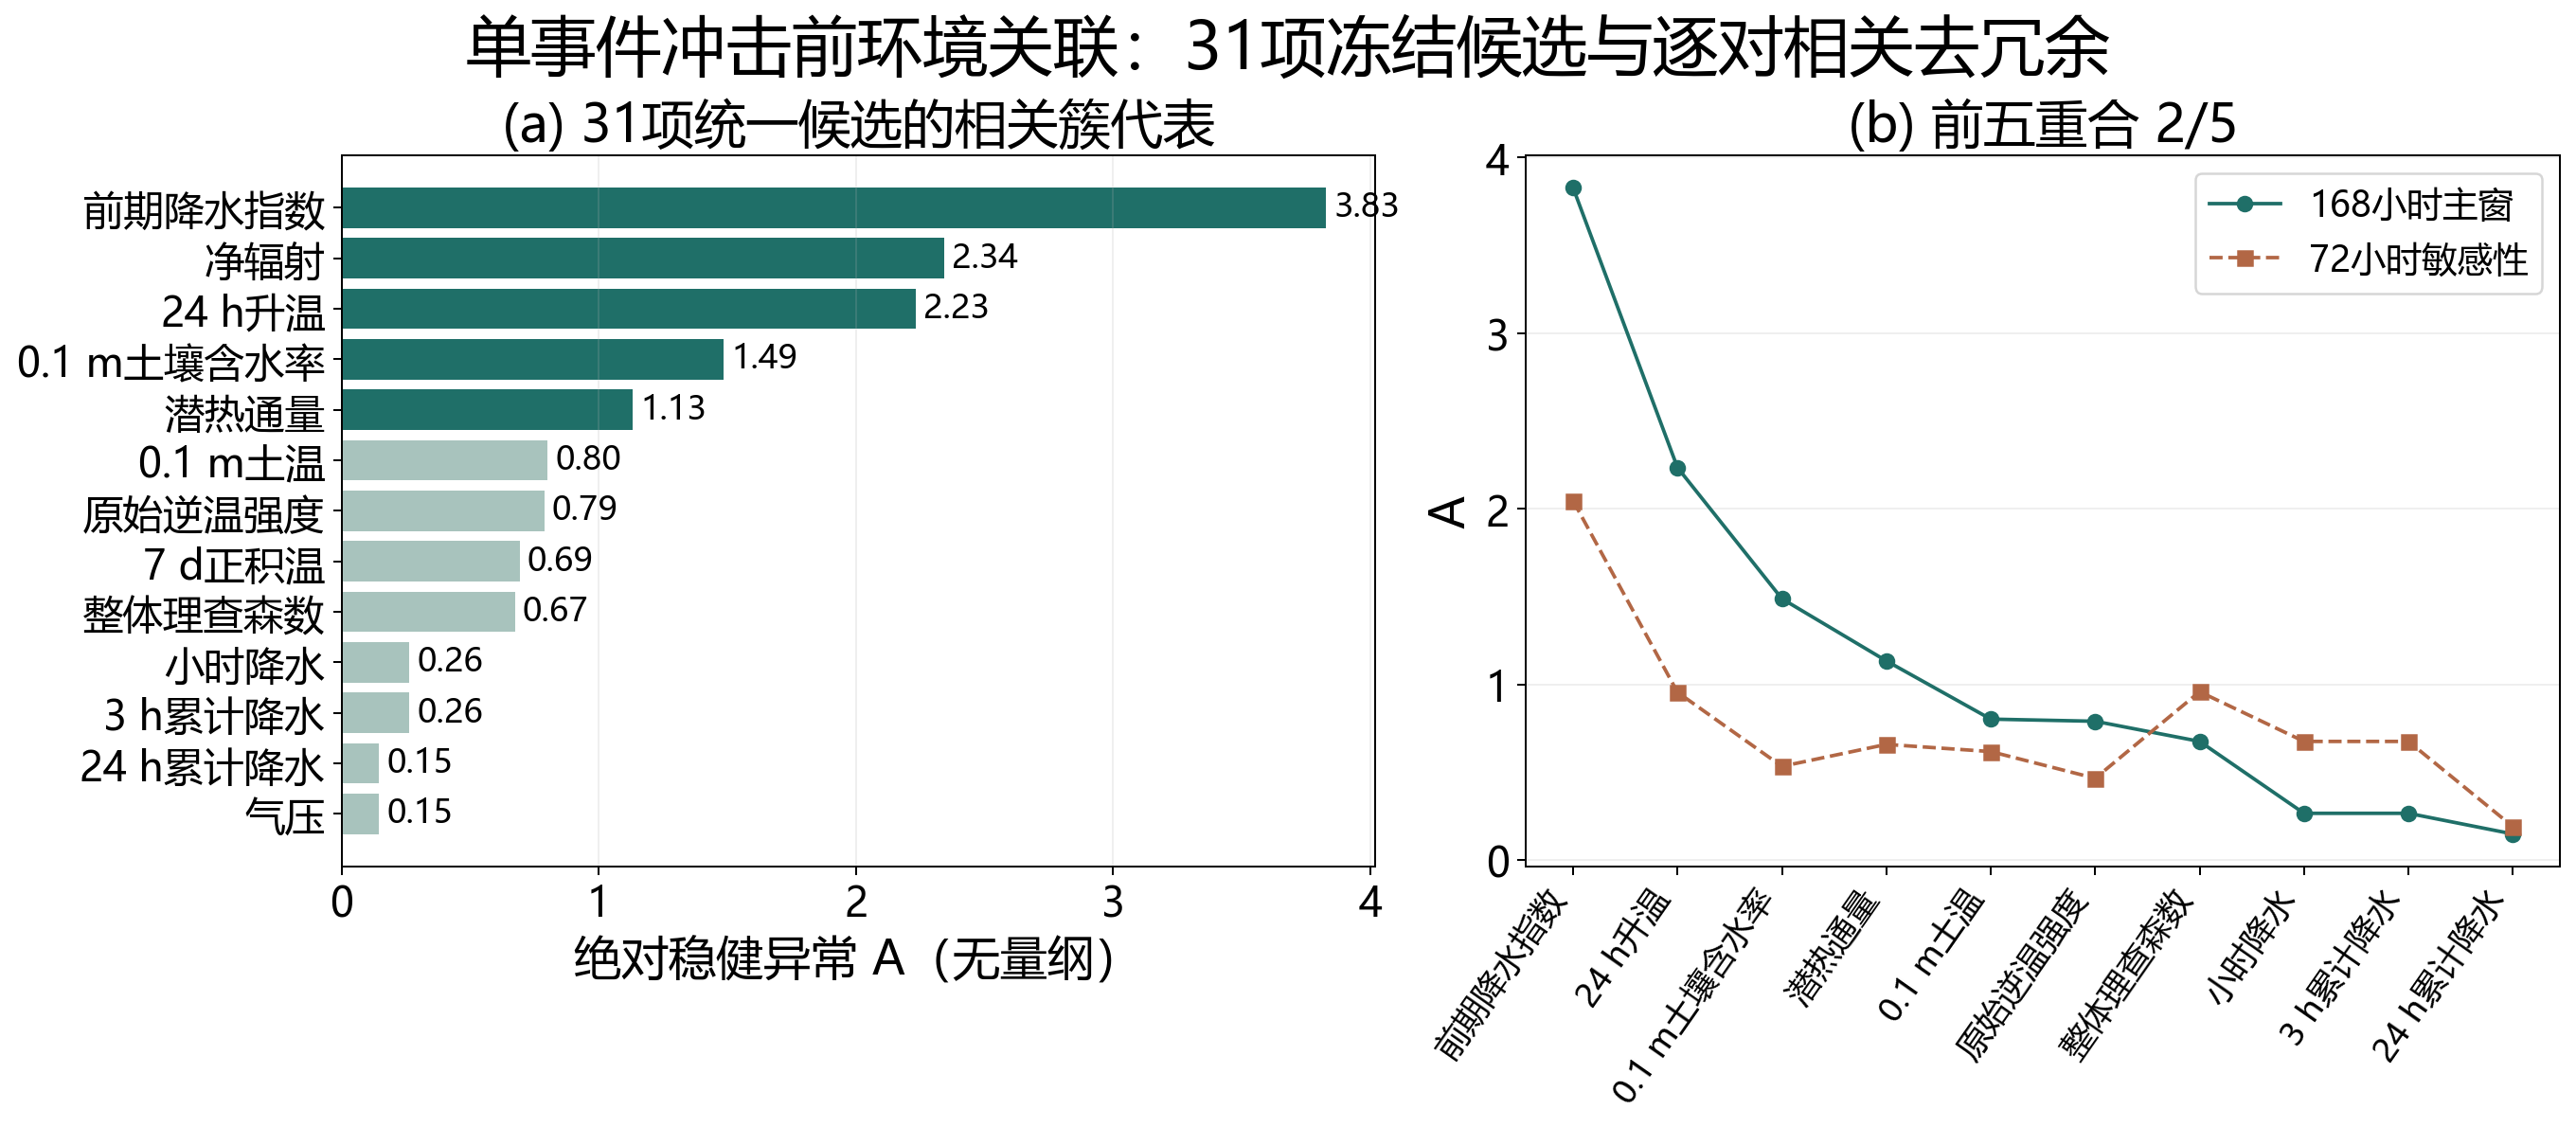
\includegraphics[width=0.84\textwidth]{figures/01c_统一候选关联.png}
\caption{31项候选关联排序与去冗余前五}
\label{fig:q1-unified}
\end{figure}

图\ref{fig:q1-unified}同时给出完整排序、相关簇和头部去冗余结果；颜色只区分观测家族，尾秩是参照窗内的描述量，不表示机制独立性。

API的事件窗均值为23.492 mm，参照中位为9.008 mm，绝对差14.484 mm，是唯一$A>3$的候选，说明本次过程前存在较持续的降水记忆。$R_n$的事件窗均值为158.479 W/m$^2$，参照中位为138.551 W/m$^2$；其所在相关簇同时含2米温湿、风切变、短波、消融能量及部分湍流通量，应把它理解为近地层能量状态的代表，而不是独立机制。24小时升温均值为0.294 $^\circ$C，参照中位为$-0.019\ ^\circ$C，反映事件窗内快速增温。0.1米土壤含水率均值0.1271，高于参照中位0.0918，表示浅层土壤水分偏湿；LE均值54.917 W/m$^2$，高于参照中位42.033 W/m$^2$。后四项的$A$均小于1.5，异常幅度明显小于API。

窗长敏感性保留了“降水记忆和升温”这一信号：72小时去冗余前五为小时消融有效能量、API、$Ri_b$、24小时升温和降水，与168小时前五重合API和24小时升温两项。留一年检查亦不完全稳定：省略2021、2023、2024年时前五重合数分别为4、3、3项；省略不同年可能使API与7日前期降水互换代表，但相关簇成员关系仍在。2025年同历日对照的最大$A=3.336817142622748$，低于本次正式头项3.8290425800714973；这表明本次头项不低于该同类日期，但单个2025日期不足以构成确证非灾样本。

\subsection{构造性对照与适用限制}
旧的26项代理榜以水源代理$Q_w$的90\%分位为标签，前五为净辐射、饱和水汽压差、2米气温、API和24小时累积降水，2021--2024训练、2025留出的AUC为0.9902。该高分首先说明水文代理可由其驱动项重建；净辐射、温度、降水和API又直接参与标签或供水构造，其排序不构成独立发现。与代理榜前五相比保留4项，全榜$\tau=0.7169$；CRITIC三列反映事件异常、强水源日判别与触发耦合之间的冲突，三列共享观测，只用于方法比较，不构成独立数据验证。因此两榜定位为构造性对照，不是本文正式前五。

正式榜的适用范围如下。第一，它是单事件环境关联；没有非灾目录，$A$不用于转换发生概率、风险比或普适排序。第二，93个参照窗来自三个有效年份，年际样本有限；尾秩受窗口重叠影响，不作为独立$p$值。第三，API、$R_n$、消融能量和LE与问题二水源模型共享观测或物理构成，榜上位置不表示独立预测能力。第四，站点代表局地近地层，不代表源区冰温和县域空间梯度。第五，相关簇去冗余只影响展示；被合并变量仍有物理意义，完整31项排序和相关边随成果保存。正式结论是：在固定候选池和同季匹配方案下，API最异常，净辐射、24小时升温、浅层土壤含水率和潜热通量随后；这五项用于解释本次事件前的环境组合，不足以单独证明因果或预测未来泥石流。
